\documentclass{article}\usepackage[]{graphicx}\usepackage[]{xcolor}
% maxwidth is the original width if it is less than linewidth
% otherwise use linewidth (to make sure the graphics do not exceed the margin)
\makeatletter
\def\maxwidth{ %
  \ifdim\Gin@nat@width>\linewidth
    \linewidth
  \else
    \Gin@nat@width
  \fi
}
\makeatother

\definecolor{fgcolor}{rgb}{0.345, 0.345, 0.345}
\newcommand{\hlnum}[1]{\textcolor[rgb]{0.686,0.059,0.569}{#1}}%
\newcommand{\hlsng}[1]{\textcolor[rgb]{0.192,0.494,0.8}{#1}}%
\newcommand{\hlcom}[1]{\textcolor[rgb]{0.678,0.584,0.686}{\textit{#1}}}%
\newcommand{\hlopt}[1]{\textcolor[rgb]{0,0,0}{#1}}%
\newcommand{\hldef}[1]{\textcolor[rgb]{0.345,0.345,0.345}{#1}}%
\newcommand{\hlkwa}[1]{\textcolor[rgb]{0.161,0.373,0.58}{\textbf{#1}}}%
\newcommand{\hlkwb}[1]{\textcolor[rgb]{0.69,0.353,0.396}{#1}}%
\newcommand{\hlkwc}[1]{\textcolor[rgb]{0.333,0.667,0.333}{#1}}%
\newcommand{\hlkwd}[1]{\textcolor[rgb]{0.737,0.353,0.396}{\textbf{#1}}}%
\let\hlipl\hlkwb

\usepackage{framed}
\makeatletter
\newenvironment{kframe}{%
 \def\at@end@of@kframe{}%
 \ifinner\ifhmode%
  \def\at@end@of@kframe{\end{minipage}}%
  \begin{minipage}{\columnwidth}%
 \fi\fi%
 \def\FrameCommand##1{\hskip\@totalleftmargin \hskip-\fboxsep
 \colorbox{shadecolor}{##1}\hskip-\fboxsep
     % There is no \\@totalrightmargin, so:
     \hskip-\linewidth \hskip-\@totalleftmargin \hskip\columnwidth}%
 \MakeFramed {\advance\hsize-\width
   \@totalleftmargin\z@ \linewidth\hsize
   \@setminipage}}%
 {\par\unskip\endMakeFramed%
 \at@end@of@kframe}
\makeatother

\definecolor{shadecolor}{rgb}{.97, .97, .97}
\definecolor{messagecolor}{rgb}{0, 0, 0}
\definecolor{warningcolor}{rgb}{1, 0, 1}
\definecolor{errorcolor}{rgb}{1, 0, 0}
\newenvironment{knitrout}{}{} % an empty environment to be redefined in TeX

\usepackage{alltt}
\usepackage{amsmath} %This allows me to use the align functionality.
                     %If you find yourself trying to replicate
                     %something you found online, ensure you're
                     %loading the necessary packages!
\usepackage{amsfonts}%Math font
\usepackage{graphicx}%For including graphics
\usepackage{hyperref}%For Hyperlinks
\usepackage[shortlabels]{enumitem}% For enumerated lists with labels specified
                                  % We had to run tlmgr_install("enumitem") in R
\hypersetup{colorlinks = true,citecolor=black} %set citations to have black (not green) color
\usepackage{natbib}        %For the bibliography
\setlength{\bibsep}{0pt plus 0.3ex}
\bibliographystyle{apalike}%For the bibliography
\usepackage[margin=0.50in]{geometry}
\usepackage{float}
\usepackage{multicol}

%fix for figures
\usepackage{caption}
\newenvironment{Figure}
  {\par\medskip\noindent\minipage{\linewidth}}
  {\endminipage\par\medskip}
\IfFileExists{upquote.sty}{\usepackage{upquote}}{}
\begin{document}

\vspace{-1in}
\title{Lab 5 -- MATH 240 -- Computational Statistics}

\author{
  Camilo \\
  Colgate University  \\
  Mathematics Department  \\
  {\tt cgranadacossio@colgate.edu}
}

\date{2/25/25}

\maketitle

\begin{multicols}{2}
\begin{abstract}
This lab applied statistical analysis techniques using \texttt{tidyverse} \citep{tidyverse} in \texttt{R} to determine which band has the largest influence on the collaborative song \textit{Allentown} by the All Get Out, The Front Bottoms, and Manchester Orchestra. Using datasets sets from \texttt{Essentia} \citep{essentia} and \texttt{LIWC} \citep{liwc}, I extract musical features to classify the song's similarity to each band. The analysis utilizes \textbf{outlier detection, summary statistics, and data visualization techniques} to provide insights
\end{abstract}

\noindent \textbf{Keywords:} Statistical analysis; Data visualization; Outlier detection; \texttt{tidyverse}; Musical feature

\section{Introduction}

In 2018, \textit{Allentown}, a collaborative song by The Front Bottoms, Manchester Orchestra, and All Get Out, was released. The goal of this lab is to determine which band contributed more significantly to the song's composition using statistical techniques. The lab focuses on extracting numerical features from \texttt{Essentia's} dataset, summarizing and comparing these features across the three bands, and using \texttt{ggplot2} \citep{gg} for visualization. By implementing boxplots, scatter plots, and summary statistics, I identified patterns that highlight \textit{Allentown's} alignment with each band's musical style.


\section{Methods}

The dataset includes key features such as \texttt{overall\textunderscore loudness, tempo, danceability, and emotion}. The function \texttt{out()} was developed to compute summary statistics and classifying outliers. This was done using \texttt{group\_by()} and \texttt{summarize()}. I computed minimum and maximum values per artist and determined the lower and upper fences ($Q\_1 - 1.5 \times IQR, Q\_3 + 1.5 \times IQR$) to detect outliers. I applied \texttt{mutate()} to indicate whether \textit{Allentown} was \textbf{out of range}, an \textbf{outlier}, or \textbf{within range}. A filtered Data Frame stored the statistical results for all the numerical features.\\

\noindent To begin the analysis of the data I used the \texttt{xtable} \citep{xtab} package to generate a summary table of numerical features. This table provides a detailed comparison of \textit{Allentown's} values against the lower and upper fences showing whether the song falls within range, is an outlier, or is out of range for each feature across the three bands.\\

\noindent Visualization of the results were created through box plots comparing \textit{Allentown's} feature values to each band's distribution and scatter plots highlighting \textit{Allentown's} placement relative to the bands. The \texttt{facet\_wrap()} function was used to arrange the plots together.


\section{Results}

The jittered scatter plots provide a visual representation of how \textit{Allentown's} musical features compare to those of the three bands. For \texttt{danceability}, \textit{Allentown's} aligns most closely with All Get Out, as indicated by its proximity to the band's typical range. The \texttt{emotion} feature, however, places \textit{Allentown} closer to The Front Bottoms. The \texttt{overall\_loudness} metric is positioned near Manchester Orchestra, but remains within the general range of all three bands. Lastly, \textit{Allentown's} tempo is most similar to The Front Bottoms, thought it is also relatively close to Manchester Orchestra. \\

\noindent The box plots further clarify the extent to which \textit{Allentown's} features deviate from each band's typical range. \texttt{Danceability} and \texttt{emotion} fall outside the interquartile range but remain within the overall spread, suggesting that \textit{Allentown} exhibits moderate stylistic differences from each band. The \texttt{overall\_loudness} and \texttt{tempo} features, on the other hand, are situated near the lower quartile across all three bands, reinforcing the idea that \textit{Allentown} blends characteristics from multiple sources rather than aligning strongly with one particular group.\\

\noindent The final bar plot categorizes \textit{Allentown's} features based on their classification as out of range, outlying, or within range. Most features fall within the expected distribution for all three bands, indicating a high level of stylistic integration. However, a small proportion of features are classified as outliers across all bands, suggesting that \textit{Allentown} introduces unique elements that differentiate it from the contributing artists' historical compositions.

\section{Discussion}

My analysis suggests that \textit{Allentown} integrates elements from all three bands. The \texttt{tempo} and \texttt{emotion} metrics are closest to The Front Bottoms and Manchester Orchestra, while \texttt{danceability} aligns more with All Get Out. The box plots, scatter plots, and summary table reinforce that \textit{Allentown} is a blend of multiple influences rather than strictly fitting within one band's historical musical style.\\

\noindent The bar plot results suggest that \textit{Allentown's} features are least out of range when compared to Manchester Orchestra's historical compositions. This implies that while elements of all three bands are present, \textit{Allentown's} overall structure and musical characteristics most closely align with Manchester Orchestra. The Front Bottoms also exhibit strong influence, particularly on \texttt{tempo} and \texttt{emotion}, while All Get Out's contribution is reflected in \texttt{danceability}. However, since Manchester Orchestra has the fewest features classified as \textquotedblleft Out of Range \textquotedblright, it is the best overall match for \textit{Allentown}. \\

\noindent Thus, based on the statistical alignment of \textit{Allentown's} primary musical attributes, Manchester Orchestra appears to have contributed the most to the song's composition, though the song retains influences from all three bands.

\begin{knitrout}\scriptsize
\definecolor{shadecolor}{rgb}{0.969, 0.969, 0.969}\color{fgcolor}
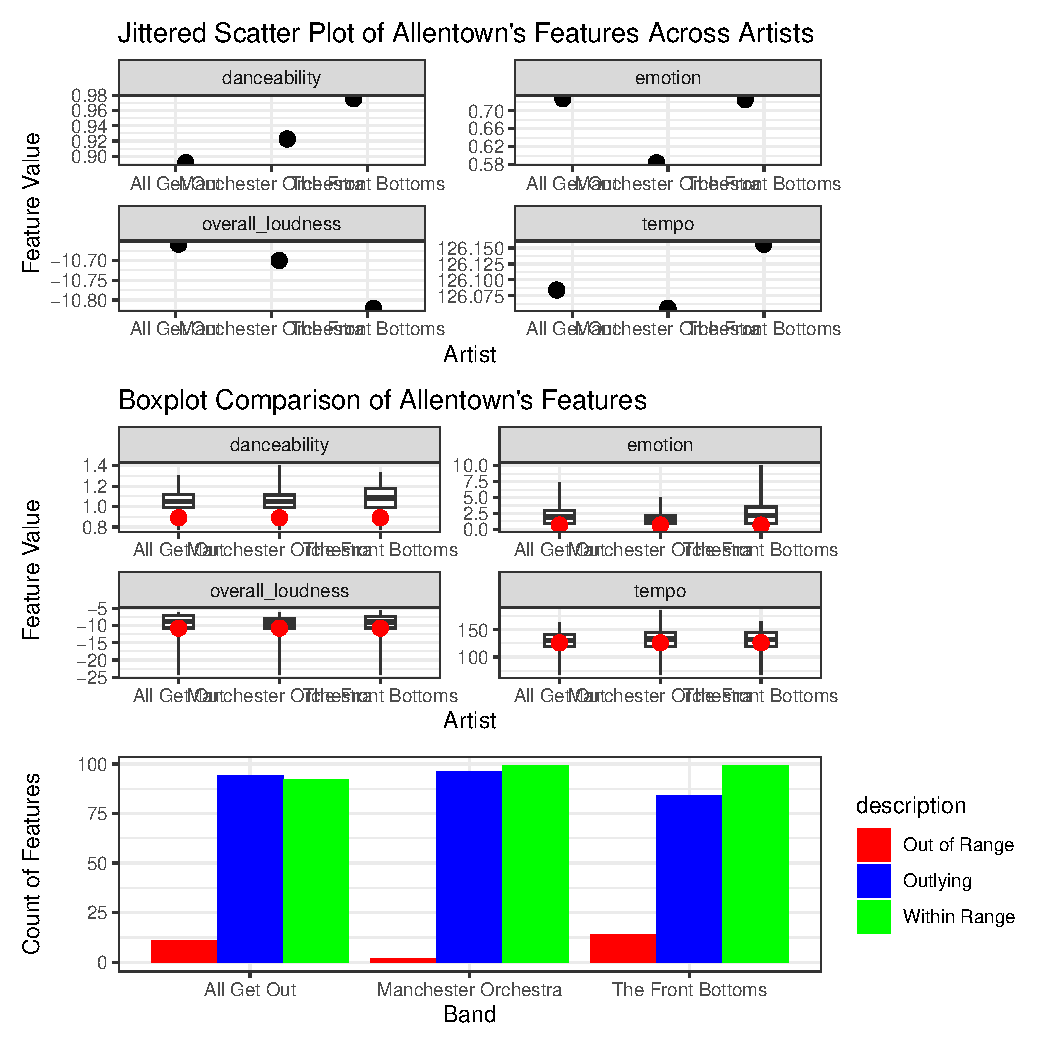
\includegraphics[width=\maxwidth]{figure/unnamed-chunk-1-1} 
\end{knitrout}

%%%%%%%%%%%%%%%%%%%%%%%%%%%%%%%%%%%%%%%%%%%%%%%%%%%%%%%%%%%%%%%%%%%%%%%%%%%%%%%%
% Bibliography
%%%%%%%%%%%%%%%%%%%%%%%%%%%%%%%%%%%%%%%%%%%%%%%%%%%%%%%%%%%%%%%%%%%%%%%%%%%%%%%%
\vspace{2em}

\begin{tiny}
\bibliography{bib}
\end{tiny}
\end{multicols}

%%%%%%%%%%%%%%%%%%%%%%%%%%%%%%%%%%%%%%%%%%%%%%%%%%%%%%%%%%%%%%%%%%%%%%%%%%%%%%%%
% Appendix
%%%%%%%%%%%%%%%%%%%%%%%%%%%%%%%%%%%%%%%%%%%%%%%%%%%%%%%%%%%%%%%%%%%%%%%%%%%%%%%%
\newpage
\onecolumn


\end{document}
